While the \foopsi filter is both efficient and effective, more powerful algorithms are available as inference techniques for the proposed models.  In particular, previously, we developed a sequential Monte Carlo (SMC; aka, particle) filter.  While the \foopsi filter obtains an approximation to the MAP estimate of the spike train, the SMC filter obtains the probability and variance of a spike occurring in each time bin.  In other words, instead of merely providing a point estimate of the distribution of spike trains, the SMC filter provides the whole distribution, but only for each time bin.  The advantage of this approach is that uncertainty is more explicitly considered, yielding improved inference accuracy.  Further, the expectation-maximization algorithm depends on the variance, so we need not approximate it (as we did in Eq. \eqref{eq:par2}) to estimate the parameters.  

However, the SMC filter is not quite as efficient as the \foopsi filter, and it requires potentially many iterations to converge to a good solution.  Therefore, finding a good initialization of the parameters is key.  Therefore, we can use the \foopsi filter to find a good set of parameters for the SMC filter, and significantly reduce the number of iterations required to converge.  Fig. \ref{fig:smc_init} shows how the SMC filter outperforms the \foopsi filter on an example cell.  Notably, the SMC filter was only iterated a few times to obtain this result, whereas without the \foopsi initialization, several fold more iterations were required.  This result is typical of all the cells we recorded from.

\begin{figure}[h!]
\centering 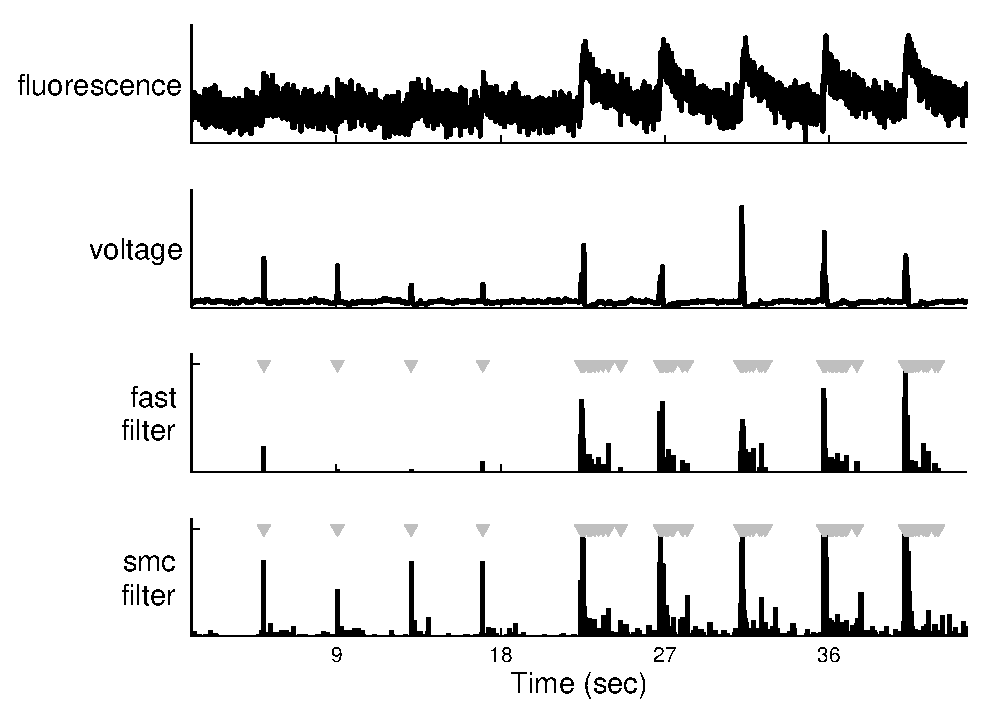
\includegraphics[width=.9\linewidth]{../figs/smc_init}
\caption{An example from adam's data.} \label{fig:smc_init}
\end{figure}